\section{Introduction}
\label{sec:introduction}
AI inference demand is expected to grow by $10{,}000\times$ over the next five
years~\citep{cra2026aifuture}. General-purpose accelerators leave significant
efficiency gains unrealized, which motivates accelerators specialized to their
target workloads. Specialization, however, requires coordinating datapaths,
memory capacity, mappings, and compiler transformations, and the resulting
design space can exceed $\mathcal O(10^{2300})$~\citep{zhang_fast}. Engineers typically explore it in
stages: choose hardware, map each operation, then optimize data reuse. Automation
accelerates these stages without necessarily removing their information loss.
A locally faster tile can consume the memory needed to retain a neighboring
tensor; a slightly slower tile can therefore yield a faster complete schedule.

We introduce \textsc{CHEETAH}: \acroletter{C}o-designed \acroletter{H}ardware
\acroletter{E}xploration via \acroletter{E}fficient \acroletter{T}hroughput and
\acroletter{H}ybrid-search. One master LP relaxation exposes these interactions
jointly. Its implementation choices determine work, traffic, and workspace;
time-indexed states track residency and reuse; and shared hardware variables
allocate compute, vector, memory, and bandwidth resources under area and power
budgets. McCormick envelopes and disaggregated epigraphs keep the model linear.
The relaxation supplies bounds for its declared domain, while integral recovery
and replay supply a concrete chip and software schedule. These are distinct
outputs: a low fractional objective alone is not an executable design.

\paragraph{One program, many architectures.}
The formulation operates on a graph of independent logical invocations and
typed storage objects. Convolutions, dense and expert GEMMs, attention, and
vector operations contribute implementation-specific coefficients and
dependencies. Optional batches and fusion groups cover original invocations
without erasing their identities. KV prefixes, expert weights, and long skip
connections enter the same capacity and readiness accounting. This makes the
program reusable across architectures without assuming that identical shapes
must share a decision.

\paragraph{Beyond prefill: the decode memory wall.}
Prefill amortizes weight traffic across many tokens; autoregressive decode
repeatedly accesses weights and an expanding KV history. Batching helps, but
sparse routing also increases the number of experts touched. Under independent
uniform top-$k$ routing, the expected union is
$n[1-(1-k/n)^B]$: with $n=256$, $k=8$, it grows from $8$ experts at batch one
to about $163$ at batch $32$. Thus batching does not guarantee a compute-bound
decode phase. CHEETAH jointly chooses resource provisioning, compatible
batches, and temporal residency. Our full-inference experiment uses actual
routes, retains the complete KV history, and charges every restore; its gains
do not assume that all weights or KV fit on chip.

\paragraph{Scaling the search.}
The complete temporal program is too large to materialize. OCS evaluates linear
operators and adjoints on compact working supports, using GPU first-order
updates, reversible scaling, and structured temporal incidence. Full-domain
checking remains separate from a working solve. An LLM architect reads resource
prices and trial diagnostics to propose implementations or search neighborhoods;
deterministic checks decide whether to admit them. The original campaign couples
this controller to Vizier; the master also admits hardware choices directly.

\paragraph{Contributions.}
\begin{enumerate}[leftmargin=*,itemsep=2pt,topsep=3pt]
\item A unified LP abstraction for hardware sizing, joint tiling--fusion,
time-indexed placement, and rematerialization, with explicit causal storage and
service constraints for full inference.
\item An operator-based solution path combining OCS, compact temporal
representations, checked bounds, and independently replayed integral recovery.
\item A diagnostic-guided LLM architect that reduces invalid trials in the
original campaign from $24.5\%$ to $5.9\%$ without replacing feasibility checks.
\item Predicted accelerator gains across vision, language, and diffusion
workloads, plus a full-input DeepSeek design with $22.88\times$ overall speedup
and matched prefill/decode feature controls. RTL and synthesis studies test
selected mechanisms; the full-task latency remains an analytical prediction.
\end{enumerate}

Section~\ref{sec:related} positions the work; Section~\ref{sec:prelim}
explains sequential information loss and relaxation. Section~\ref{sec:methods}
presents the master and its feature encodings, and Section~\ref{sec:ocs} describes
OCS. Section~\ref{sec:experiments} reports the original campaign and the full-input
phase and feature results. The appendix provides complete rows, containment
arguments, physical-validation details, economics, and reproduction evidence.


% ---- plots restored from the long version, original placement ----

\begin{figure}[ht!]
    \centering
    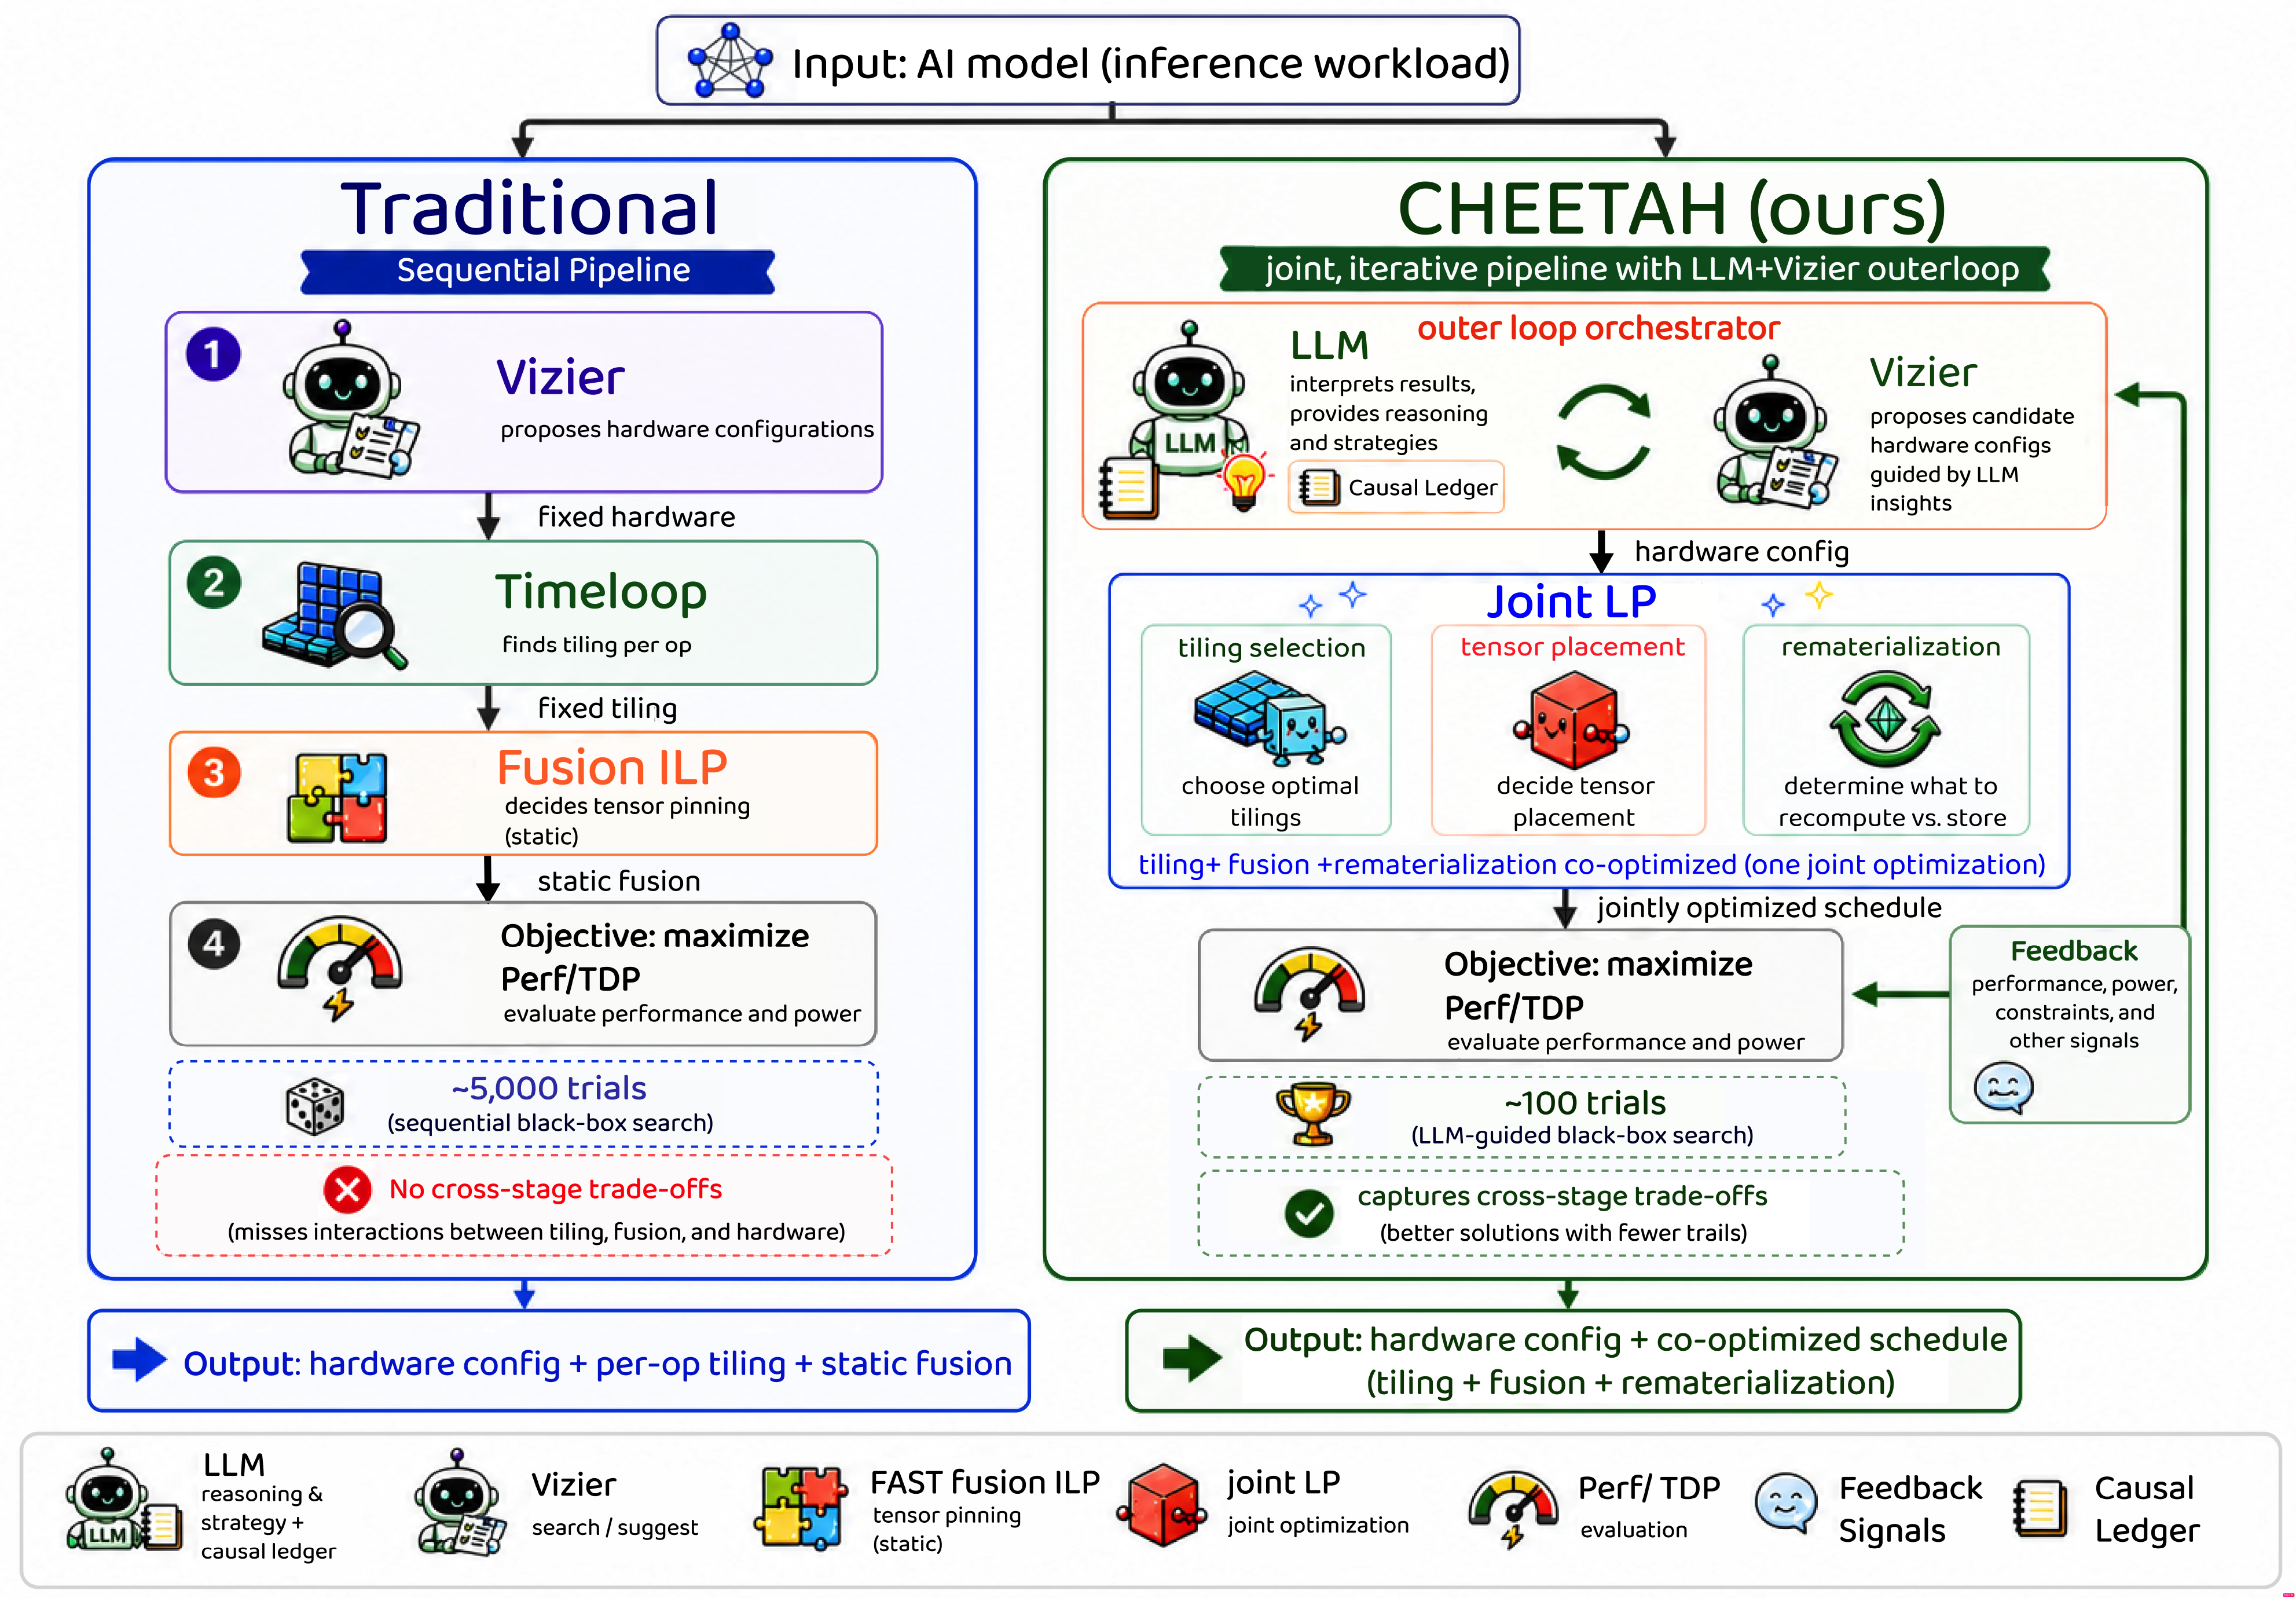
\includegraphics[width=1.0\linewidth]{figs/cheetah_v4_new.png}
\caption{Sequential vs Our Unified Optimization Paradigm.
(Left) Baseline methods decouple hardware search, operation-level tiling, and static fusion; precluding cross-stage trade-offs.
(Right) CHEETAH presents a unified LLM-driven LP-solver-based framework that jointly optimizes tiling, placement, and rematerialization while learning from a causal ledger.}
\label{fig::workflow}
\end{figure}

\begin{figure}[ht!]
    \centering
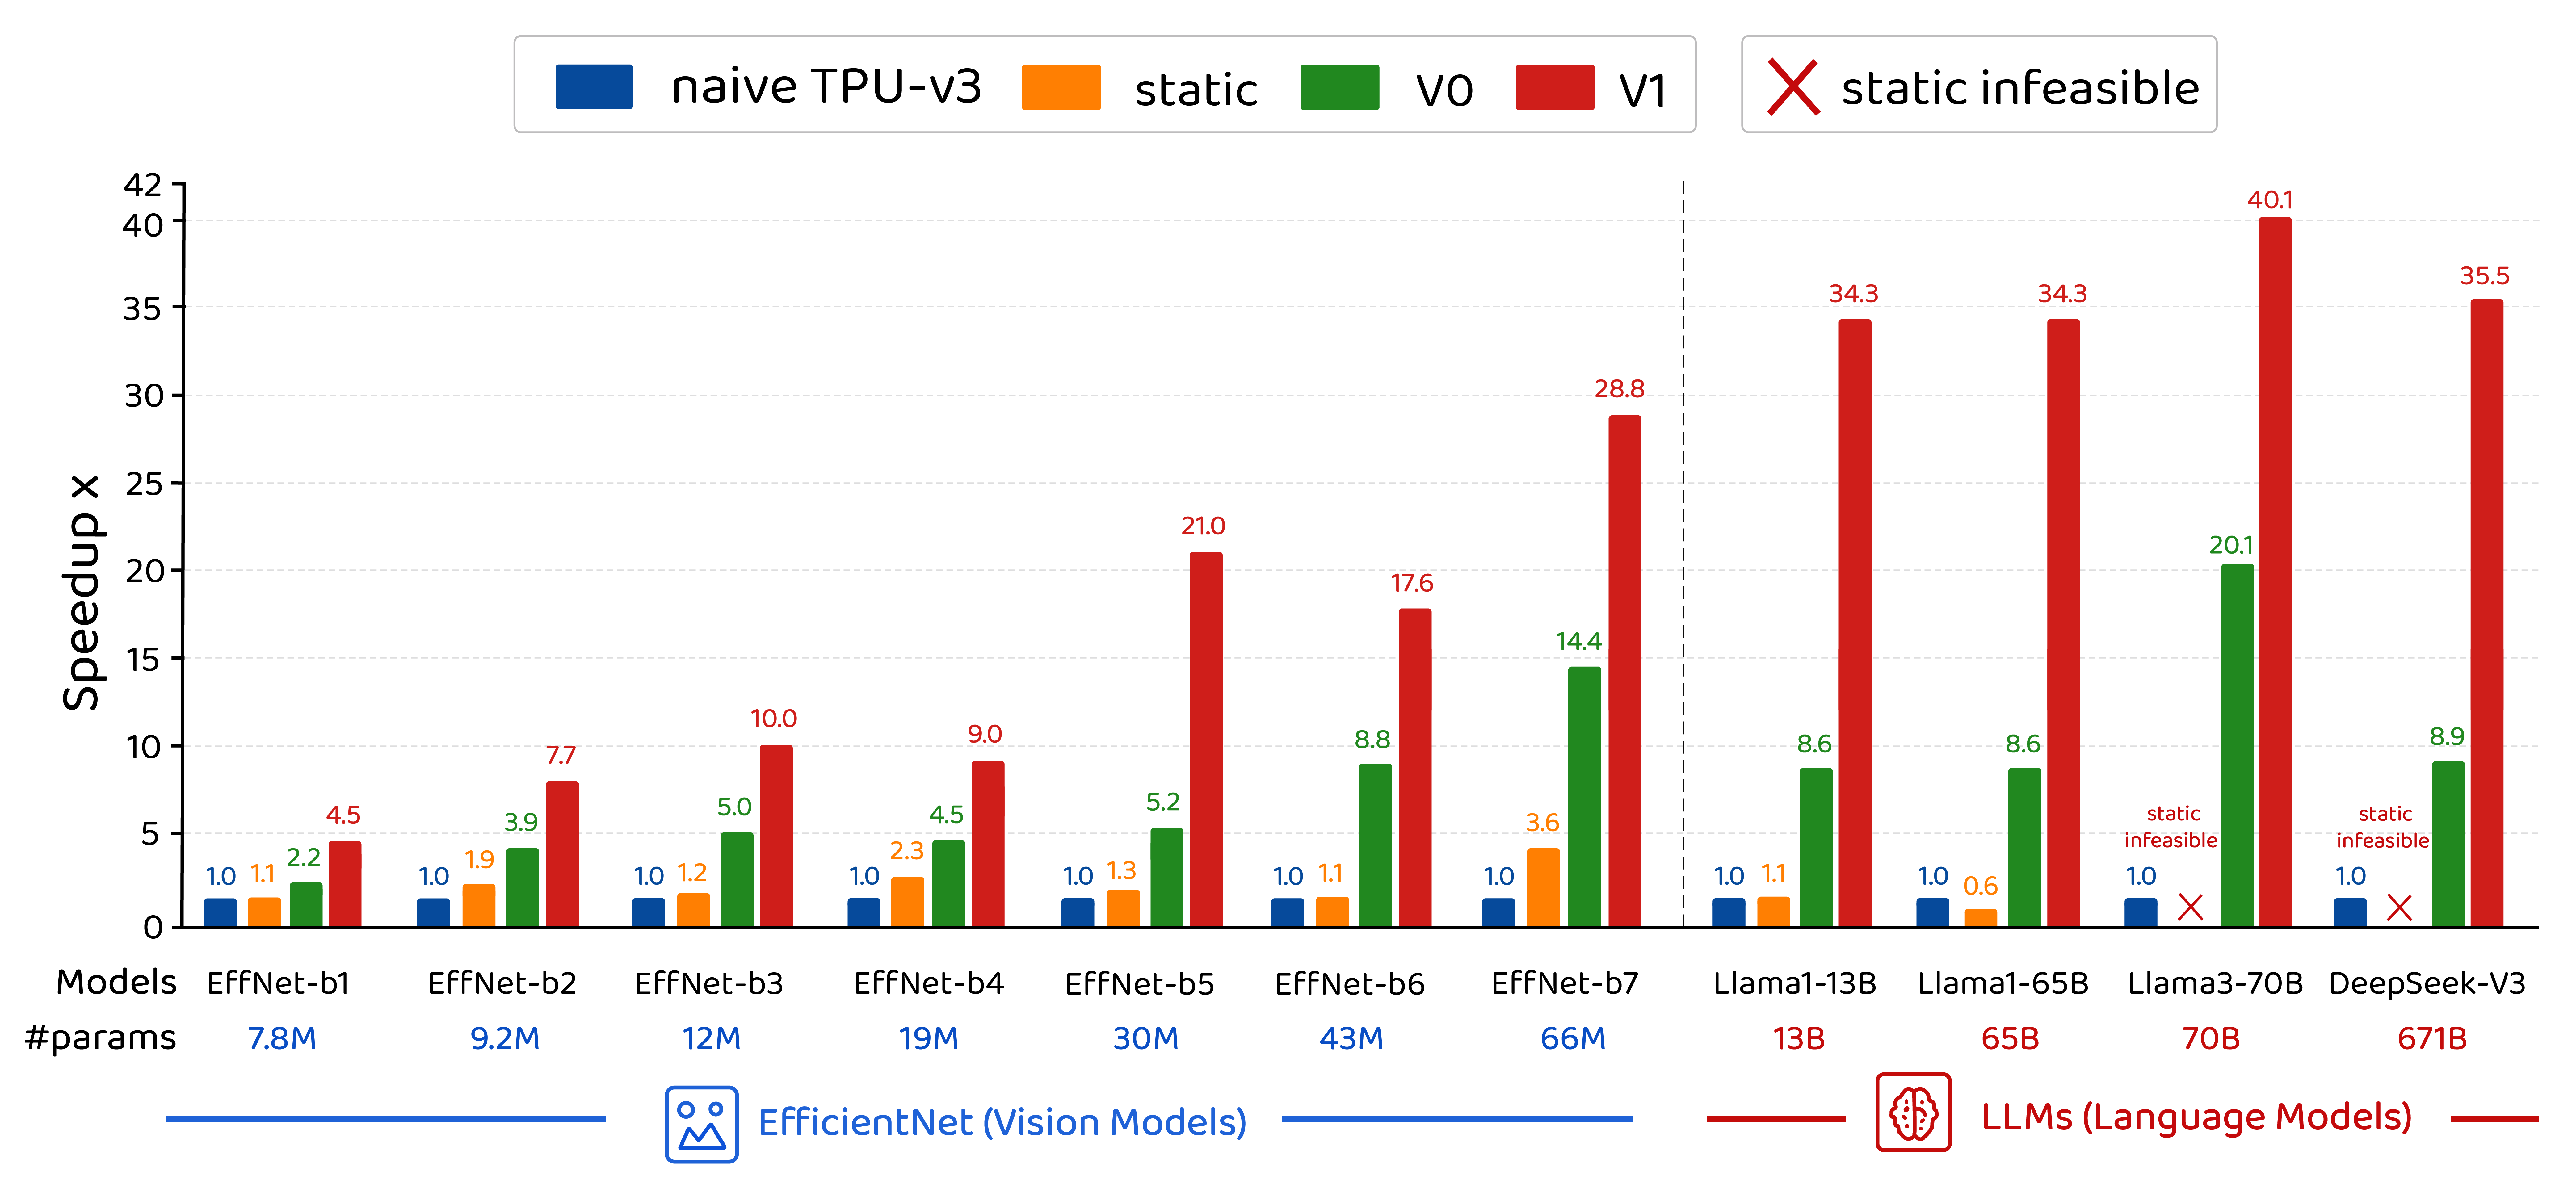
\includegraphics[width=1.0\linewidth]{fig3/speedup_final_v3.png}
\caption{Speedup over modeled TPU-v3 baseline for each workload and formulation: CHEETAH-V1's joint tiling-fusion optimization achieves up to $\sim$40.1$\times$ acceleration, while static fusion is infeasible on large-scale LLMs. Progressive gains are visible across formulations: V0's dynamic placement improves over static by $2$--$20\times$, while V1's joint tiling-fusion adds another $2$--$4\times$ on top. See Section~\ref{sec:experiments} for full analysis and wall-clock time breakdowns.}
\label{fig:speedup}
\end{figure}
